\documentclass[xcolor=svgnames]{beamer}\usepackage[]{graphicx}\usepackage[]{color}
%% maxwidth is the original width if it is less than linewidth
%% otherwise use linewidth (to make sure the graphics do not exceed the margin)
\makeatletter
\def\maxwidth{ %
  \ifdim\Gin@nat@width>\linewidth
    \linewidth
  \else
    \Gin@nat@width
  \fi
}
\makeatother

\definecolor{fgcolor}{rgb}{0.345, 0.345, 0.345}
\newcommand{\hlnum}[1]{\textcolor[rgb]{0.686,0.059,0.569}{#1}}%
\newcommand{\hlstr}[1]{\textcolor[rgb]{0.192,0.494,0.8}{#1}}%
\newcommand{\hlcom}[1]{\textcolor[rgb]{0.678,0.584,0.686}{\textit{#1}}}%
\newcommand{\hlopt}[1]{\textcolor[rgb]{0,0,0}{#1}}%
\newcommand{\hlstd}[1]{\textcolor[rgb]{0.345,0.345,0.345}{#1}}%
\newcommand{\hlkwa}[1]{\textcolor[rgb]{0.161,0.373,0.58}{\textbf{#1}}}%
\newcommand{\hlkwb}[1]{\textcolor[rgb]{0.69,0.353,0.396}{#1}}%
\newcommand{\hlkwc}[1]{\textcolor[rgb]{0.333,0.667,0.333}{#1}}%
\newcommand{\hlkwd}[1]{\textcolor[rgb]{0.737,0.353,0.396}{\textbf{#1}}}%

\usepackage{framed}
\makeatletter
\newenvironment{kframe}{%
 \def\at@end@of@kframe{}%
 \ifinner\ifhmode%
  \def\at@end@of@kframe{\end{minipage}}%
  \begin{minipage}{\columnwidth}%
 \fi\fi%
 \def\FrameCommand##1{\hskip\@totalleftmargin \hskip-\fboxsep
 \colorbox{shadecolor}{##1}\hskip-\fboxsep
     % There is no \\@totalrightmargin, so:
     \hskip-\linewidth \hskip-\@totalleftmargin \hskip\columnwidth}%
 \MakeFramed {\advance\hsize-\width
   \@totalleftmargin\z@ \linewidth\hsize
   \@setminipage}}%
 {\par\unskip\endMakeFramed%
 \at@end@of@kframe}
\makeatother

\definecolor{shadecolor}{rgb}{.97, .97, .97}
\definecolor{messagecolor}{rgb}{0, 0, 0}
\definecolor{warningcolor}{rgb}{1, 0, 1}
\definecolor{errorcolor}{rgb}{1, 0, 0}
\newenvironment{knitrout}{}{} % an empty environment to be redefined in TeX

\usepackage{alltt}
\usetheme{Boadilla}
\usecolortheme[named=SeaGreen]{structure}
\usepackage{graphicx}
\usepackage{breqn}
\usepackage{xcolor}
\usepackage{booktabs}
\usepackage{verbatim}
\definecolor{links}{HTML}{2A1B81}
\hypersetup{colorlinks,linkcolor=links,urlcolor=links}
\usepackage{pgfpages}
\usepackage{listings}

%\usepackage{color}
\lstset{
language=R,                     % the language of the code
%basicstyle=\footnotesize,       % the size of the fonts that are used for the code
%numbers=left,                   % where to put the line-numbers
%numberstyle=\tiny\color{gray},  % the style that is used for the line-nxumbers
%stepnumber=1,                   % the step between two line-numbers. If it's 1, each line
% will be numbered
%numbersep=5pt,                  % how far the line-numbers are from the code
backgroundcolor=\color{white},  % choose the background color. You must add \usepackage{color}
showspaces=false,               % show spaces adding particular underscores
showstringspaces=false,         % underline spaces within strings
showtabs=false,                 % show tabs within strings adding particular underscores
%frame=single,                   % adds a frame around the code
rulecolor=\color{black},        % if not set, the frame-color may be changed on line-breaks within not-black text (e.g. commens (green here))
tabsize=2,                      % sets default tabsize to 2 spaces
captionpos=b,                   % sets the caption-position to bottom
breaklines=true,                % sets automatic line breaking
breakatwhitespace=true,         % sets if automatic breaks should only happen at whitespace
%title=\lstname,                 % show the filename of files included with \lstinputlisting;
% also try caption instead of title
keywordstyle=\color{blue},      % keyword style
commentstyle=\color{ForestGreen},   % comment style
%stringstyle=\color{black},      % string literal style
escapeinside={\%*}{*)},         % if you want to add a comment within your code
morekeywords={*,...}            % if you want to add more keywords to the set
}

\newcommand{\ShowSexpr}[1]{\texttt{{\char`\\}Sexpr\{#1\}}}

\usepackage{amsfonts, amsmath, hanging, hyperref, parskip, times}
%\usepackage[numbers]{natbib}

\usepackage[backend=bibtex,
firstinits=true,
style=authoryear,
dashed=false,
natbib=true,
doi=false,
isbn=false,
url=false,
uniquename=false,
uniquelist=false,
sorting=none,
maxcitenames=2]{biblatex}
\addbibresource{ggRandomForest.bib}

\ifx\hypersetup\undefined
\AtBeginDocument{%
\hypersetup{unicode=true,pdfusetitle,
bookmarks=true,bookmarksnumbered=false,bookmarksopen=false,
breaklinks=false,pdfborder={0 0 0},backref=false,colorlinks=false}
}
\else
\hypersetup{unicode=true,pdfusetitle,
bookmarks=true,bookmarksnumbered=false,bookmarksopen=false,
breaklinks=false,pdfborder={0 0 0},backref=false,colorlinks=false}
\fi

% \usetheme{CambridgeUS}
% \usecolortheme{seahorse}

\title{Survival in Random Forests}
%\subtitle{The ggRandomForests package}
\author[J. Ehrlinger]{John Ehrlinger}
\institute[Cleveland Clinic] % (optional)
{
Department of Quantitative Health Sciences\\
Lerner Research Institute\\
Cleveland Clinic\\
john.ehrlinger@gmail.com
}
\date[\today]



\IfFileExists{upquote.sty}{\usepackage{upquote}}{}
\begin{document}
\frame{\titlepage}
%==================================================================================
%==================================================================================

\begin{frame}
\frametitle{Random Forest}

Mature statistical ``machine learning'' method for
\begin{itemize}
\item Regression (continuous outcomes)
\item Classification (categorical outcomes)
\item Survival (time to event outcomes)
\item Others (competing risk, unsupervised, etc.)
\end{itemize}

Similar to C4.5

\end{frame}



%'
%' \end{frame}
%' %==================================================================================
%' \begin{frame}
%' \frametitle{Growing a Decision Tree}
%'


%'
%' \end{frame}
%' %==================================================================================
%' \begin{frame}
%' \frametitle{Growing a Decision Tree}
%'


%'
%' \end{frame}
%' %==================================================================================
%' \begin{frame}
%' \frametitle{Growing a Decision Tree}


%' \end{frame}
%'
%' %==================================================================================
%' \begin{frame}
%' \frametitle{Growing a Decision Tree}
%' Stopping Rule defines Terminal Nodes
%' \begin{itemize}
%' \item Minimal number of members
%' \item Homogeneity
%' \end{itemize}
%'
%' Defaults depend on the problem domain
%'
%' \begin{itemize}
%' \item Regression - min 5 unique cases
%' \item Classification - homogeneous node (min of 1)
%' \item Survival - min 3 unique cases
%' \end{itemize}
%'
%' \end{frame}
%' %==================================================================================
%' \begin{frame}
%' \frametitle{Testing a Decision Tree}
%'
%' Tree sorts each observation into a unique terminal nodes
%'
%' Test the tree with oob data.
%' \begin{itemize}
%' \item Sort test observations into terminal nodes
%'   \item Predict from training observations
%'   \item Compare with test response
%' \end{itemize}
%'
%' \end{frame}
%' %==================================================================================
%' \begin{frame}
%' \frametitle{Testing a Decision Tree}
%'
%' << decisionTree>>=
%' decTree
%' @
%'
%' \end{frame}
%' %==================================================================================
%' \begin{frame}
%' \frametitle{Decision Tree Prediction}
%'
%' Defined by terminal node membership.
%' \begin{itemize}
%' \item Fit a model to training set members
%' \item Predict from model
%' \end{itemize}
%'
%' One model for each terminal node within the tree.
%'
%' Depends on the problem domain
%' \begin{itemize}
%' \item Regression - mean value
%' \item Classification - probability of class membership
%' \item Survival - Kaplan--Meier estimates
%' \end{itemize}
%'
%' \end{frame}
%' %==================================================================================
%' \begin{frame}
%' \frametitle{Random Forest Trees}
%'
%' A forest of independent decision trees
%'
%' \begin{itemize}
%' \item Independent bootstrap training data
%' \item Add extra randomization step
%' \end{itemize}
%'
%' At each node split, RF randomly selects a subset (mtry $\le p$) of candidate variables for the split rule optimization
%'
%' Default depends on the problem domain
%'
%' \begin{itemize}
%' \item Regression - mtry = ceiling$(p/3)$
%' \item Classification - mtry = ceiling$(\sqrt{p})$
%' \item Survival - mtry = ceiling$(\sqrt{p})$
%' \end{itemize}
%'
%' \end{frame}
%' %==================================================================================
%' \begin{frame}
%' \frametitle{Random Forest Prediction}
%'
%' A forest of independent decision trees
%'
%' \begin{itemize}
%' \item Observations in a terminal node have the same predicted outcome
%' \item Bagging (Bootstrap Aggregation) over all trees
%' \end{itemize}
%'
%' Default depends on the problem domain
%'
%' \begin{itemize}
%' \item Regression - average estimates
%' \item Classification - voting or average probabilty
%' \item Survival - average survival estimates
%' \end{itemize}
%'
%' \end{frame}
%' %==================================================================================
%' \begin{frame}
%' \frametitle{Random Forest Performance}
%'
%' Measure of generalization error
%'
%' \begin{itemize}
%' \item oob data used to calculate forest prediction error
%' \end{itemize}
%' Depends on the problem domain
%' \begin{itemize}
%' \item Regression - MSE
%' \item Classification - Misclassification error
%' \item Survival - Harrell's concordance index
%' \end{itemize}
%' \end{frame}
%==================================================================================
\begin{frame}
\frametitle{Breiman's Two Cultures}

Machine Learning vs. Statistics

Machine Learning:

\begin{itemize}
\item Prediction, Prediction, Prediction
\item Black box modeling
\end{itemize}

Statistics:
\begin{itemize}
\item Why?
\item Information on underlying process
\end{itemize}

Random Forest:

\begin{itemize}
\item Why not both?
\item Insight into the black box of prediction
\end{itemize}
\end{frame}

%==================================================================================
\begin{frame}
\frametitle{Example}
Primary Biliary Cirrhosis (PBC) of the liver data set

(Fleming and Harrington 1991)

Randomized  trial of D-penicillamine (DPCA) at Mayo Clinic

312 patients from 1974 to 1984
\begin{itemize}
\item 125 deaths
\item 17 variables
\end{itemize}

\end{frame}
%' %==================================================================================
%' \begin{frame}
%' \frametitle{Example}
%'
%' PBC Cox proportional hazard model
%'
%' <<fh-model>>=
%' ## Not displayed ##
%' # Create a table summarizing the ph model from fleming and harrington 1991
%' fleming.table <- data.frame(matrix(ncol = 4, nrow = 5))
%' fleming.table[,1] <-
%'   c("Age", "log(Albumin)", "log(Bilirubin)", "Edema", "log(Prothrombin Time)")
%' colnames(fleming.table) <- c("Variables","Coef.", "Std. Err.", "Z stat.")
%' fleming.table[,2] <- c(0.0333, -3.0553,0.8792, 0.7847, 3.0157)
%' fleming.table[,3] <- c(0.00866, 0.72408,0.09873,0.29913,1.02380)
%' fleming.table[,4] <- c(3.84,-4.22,8.9,2.62,2.95)
%'
%' kable(fleming.table,
%'       row.names=NA,
%'       format="latex",
%'       digits = 3,
%'       booktabs=TRUE)
%' @
%' \end{frame}
%==================================================================================
\begin{frame}
\frametitle{Random Survival Forest}

\begin{knitrout}\footnotesize
\definecolor{shadecolor}{rgb}{0.969, 0.969, 0.969}\color{fgcolor}

{\centering 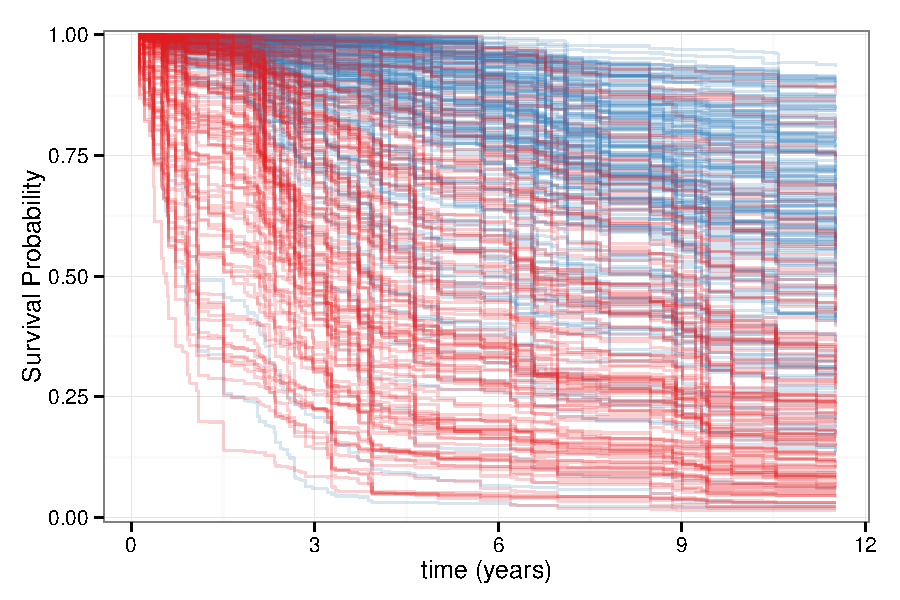
\includegraphics[width=.9\linewidth]{figures/pbc-forest-1} 

}



\end{knitrout}
\end{frame}
%' %==================================================================================
%' \begin{frame}
%' \frametitle{Random Survival Forest}
%'
%' << pbd-treatment>>=
%' gg_plt <-  plot(gg_rfsrc(rfsrc_pbc, by="treatment")) +
%'   theme(legend.position = c(.2,.2)) +
%'   labs(y = "Survival Probability", x = "time (years)",
%'        color="Treatment", fill="Treatment")+
%'   scale_color_brewer(palette="Set1")+
%'   coord_cartesian(y = c(-.01,1.01))
%' gg_plt
%' @
%' \end{frame}

%==================================================================================
\begin{frame}
\frametitle{Variable (Feature) Selection}

Two independent ranking methods

Variable IMPortance (VIMP)

\begin{itemize}
\item Based on RF Prediction Error
\item Measures the impact of variable misspecification
\end{itemize}

Minimal Depth

\begin{itemize}
\item Property of decision tree construction
\item Measures how a variable segments nodes
\end{itemize}
\end{frame}
% %==================================================================================
% \begin{frame}
% \frametitle{Variable Selection - VIMP}
%
% Prediction error (PE) estimate from oob data
%
% For each variable:
% \begin{itemize}
% \item  Randomize values within the variable
% \item Predict with randomized data
% \item Calculate a New Prediction Error estimate (NPE)
% \end{itemize}
%
% VIMP = PE - NPE
% \begin{itemize}
% \item Positive value: important in reducing error
% \item Near zero: no impact on prediction
% \item Negative value: noise variable
% \end{itemize}
% \end{frame}
%==================================================================================
\begin{frame}
\frametitle{Variable Selection - VIMP}
\begin{knitrout}\footnotesize
\definecolor{shadecolor}{rgb}{0.969, 0.969, 0.969}\color{fgcolor}

{\centering 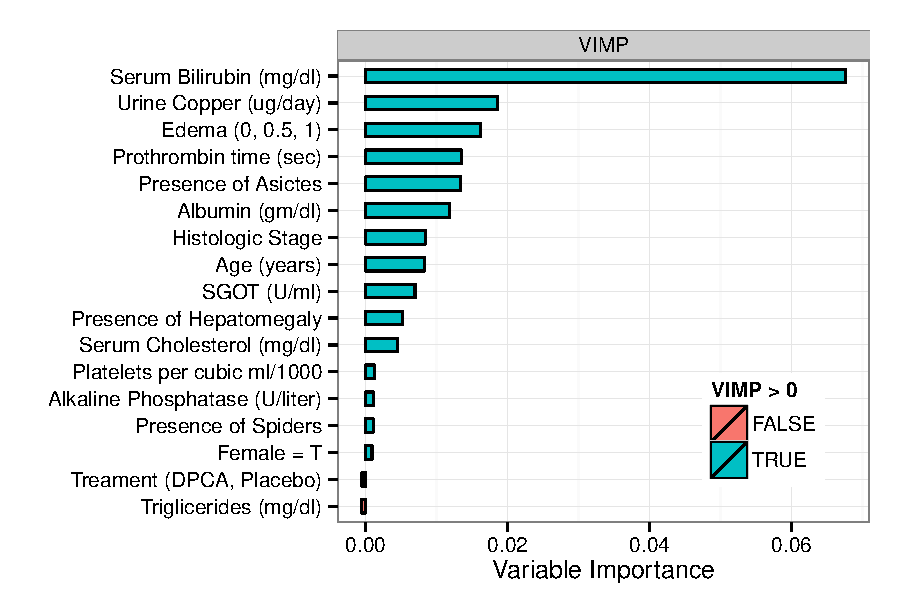
\includegraphics[width=.9\linewidth]{figures/rf-pbc-vimp-1} 

}



\end{knitrout}
\end{frame}
% %==================================================================================
% \begin{frame}
% \frametitle{Variable Selection - Minimal Depth}
%
% Within each tree
% \begin{itemize}
% \item  Number the node split levels
% \item Find the minimum split level for each variable
% \end{itemize}
%
% \end{frame}
%==================================================================================
\begin{frame}
\frametitle{Variable Selection - Minimal Depth}
\begin{knitrout}\footnotesize
\definecolor{shadecolor}{rgb}{0.969, 0.969, 0.969}\color{fgcolor}

{\centering 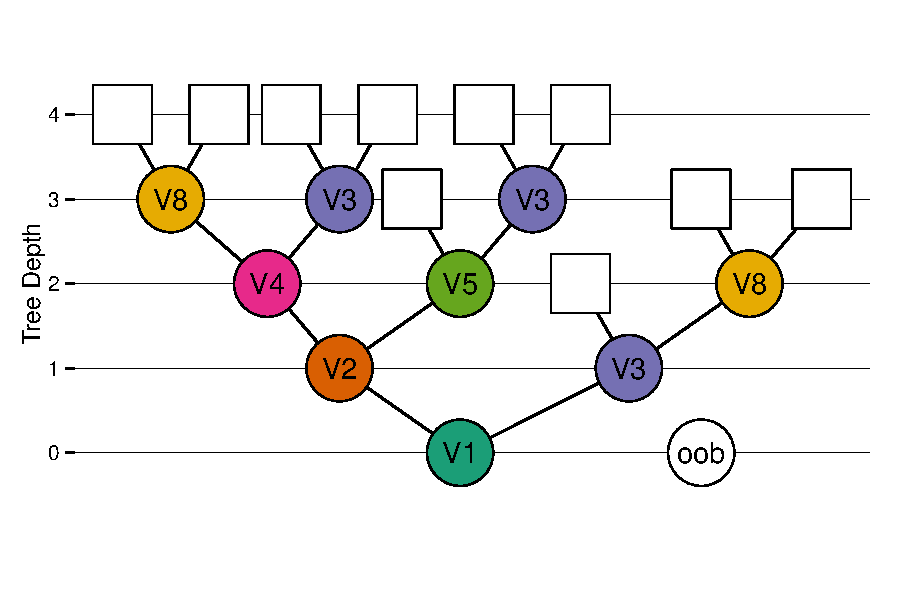
\includegraphics[width=.9\linewidth]{figures/treeDepth-1} 

}



\end{knitrout}
\end{frame}
%==================================================================================
% \begin{frame}
% \frametitle{Variable Selection - Minimal Depth}
%
% Average minimal split levels
% \begin{itemize}
% \item  each variable
%   \item over the forest
% \end{itemize}
%
% Lower values split largest nodes
% \end{frame}
%==================================================================================
\begin{frame}
\frametitle{Variable Selection - Minimal Depth}
\begin{knitrout}\footnotesize
\definecolor{shadecolor}{rgb}{0.969, 0.969, 0.969}\color{fgcolor}

{\centering 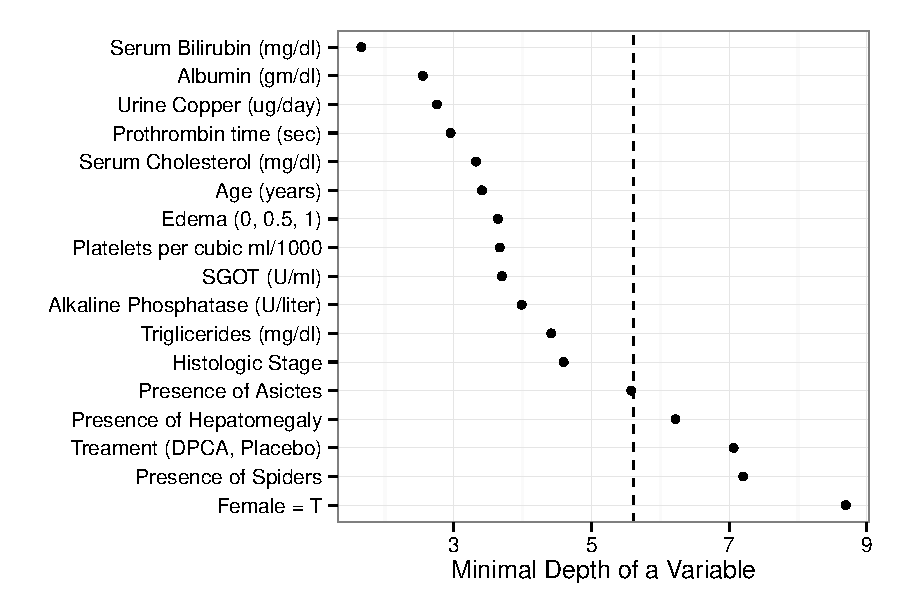
\includegraphics[width=.9\linewidth]{figures/mindepth-pbc-1} 

}



\end{knitrout}
\end{frame}
%==================================================================================
\begin{frame}
\frametitle{Random Forest}
Which variables contribute to forest prediction?
\begin{itemize}
\item  ``Stacking'' VIMP and Minimal Depth
\end{itemize}

How does response depend on variables?
\begin{itemize}
\item  Variable Dependence - Observation Based
\item  Partial Dependence - Population Based
\end{itemize}
\end{frame}

%==================================================================================
\begin{frame}
\frametitle{Variable Dependence}

Observation based

\begin{knitrout}\footnotesize
\definecolor{shadecolor}{rgb}{0.969, 0.969, 0.969}\color{fgcolor}

{\centering 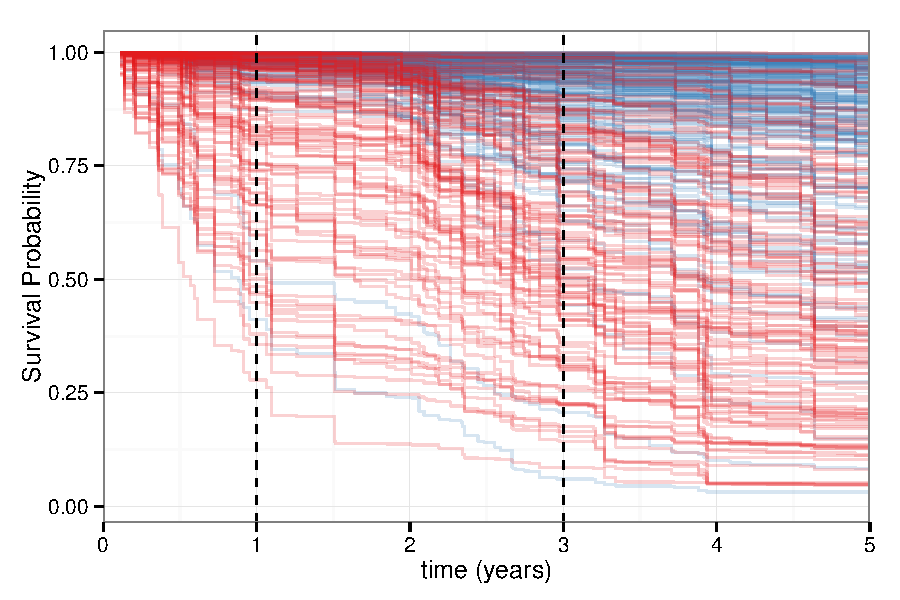
\includegraphics[width=.9\linewidth]{figures/rfsrc-plot3Mnth-pbc-1} 

}



\end{knitrout}

\end{frame}
%==================================================================================
\begin{frame}
\frametitle{Variable Dependence}

\begin{knitrout}\footnotesize
\definecolor{shadecolor}{rgb}{0.969, 0.969, 0.969}\color{fgcolor}

{\centering 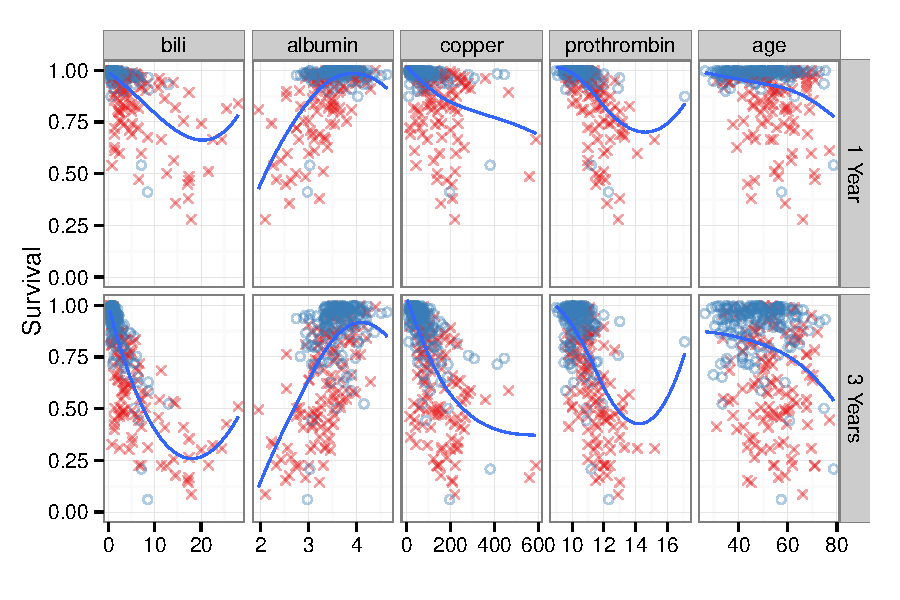
\includegraphics[width=.9\linewidth]{figures/variable-plot-pbc-1} 

}



\end{knitrout}
\end{frame}
%==================================================================================
% \begin{frame}
% \frametitle{Partial Dependence}
%
% Population Based
%
% \begin{itemize}
% \item  Create nomograms for each observation
% \begin{itemize}
% \item  Across values of variable of interest
%     \item At selected times for survival
% \end{itemize}
%   \item Average response
% \end{itemize}
% \end{frame}

%==================================================================================
\begin{frame}
\frametitle{Partial Dependence}

\begin{knitrout}\footnotesize
\definecolor{shadecolor}{rgb}{0.969, 0.969, 0.969}\color{fgcolor}

{\centering 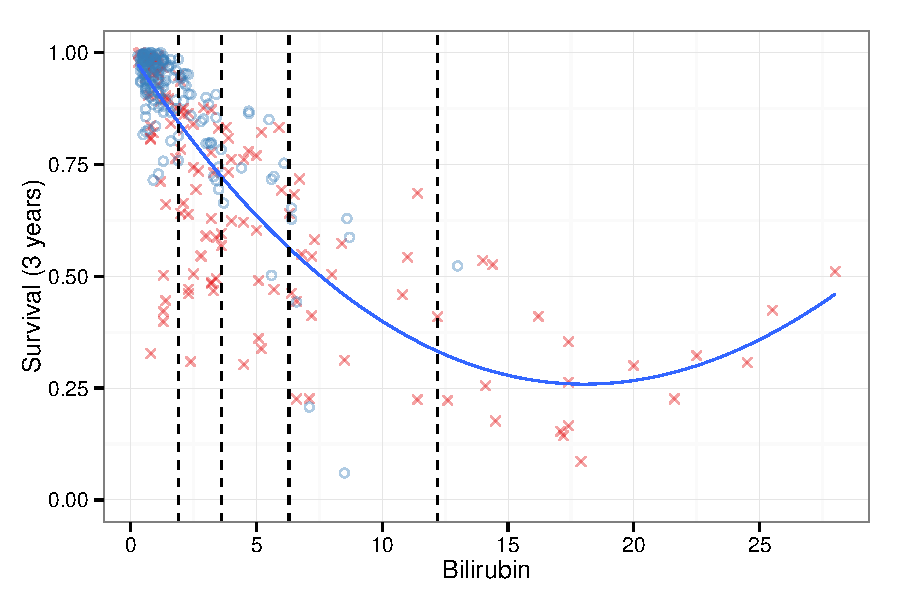
\includegraphics[width=.9\linewidth]{figures/rfs-points-1} 

}



\end{knitrout}
\end{frame}
%==================================================================================
\begin{frame}
\frametitle{Partial Dependence}

\begin{knitrout}\footnotesize
\definecolor{shadecolor}{rgb}{0.969, 0.969, 0.969}\color{fgcolor}

{\centering 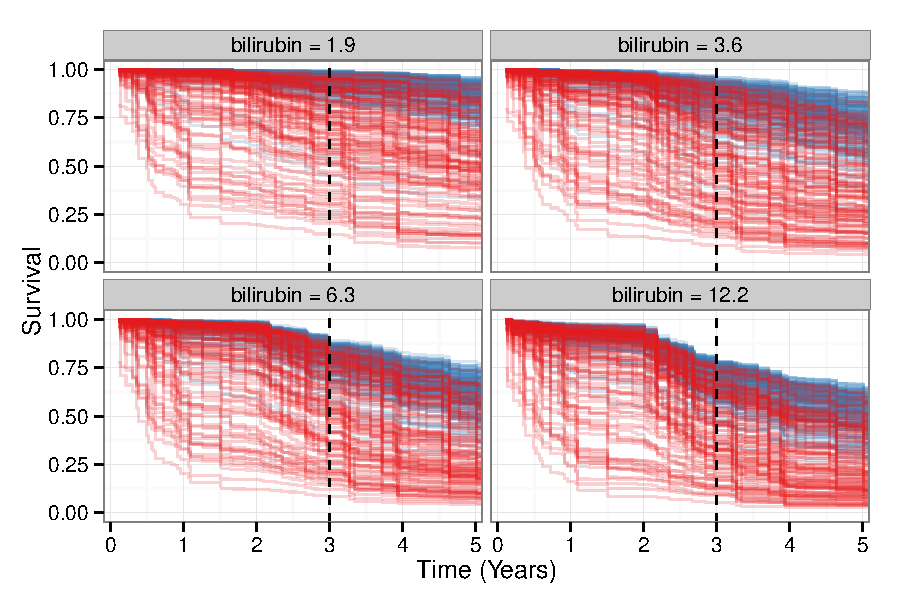
\includegraphics[width=.9\linewidth]{figures/rfs-nomo-1} 

}



\end{knitrout}
\end{frame}
%==================================================================================
%' \begin{frame}
%' \frametitle{Partial Dependence}
%'
%' << nomogram-vdep>>=
%' ggvd <- lapply(prd, function(st){
%'   indx <- which(rfsrc_pbc$time.interest >3)[1] - 1
%'   ss <- data.frame(yhat=st$survival[,indx])
%'   ss$ptid <- 1:nrow(ss)
%'   ss$cens <- rfsrc_pbc$yvar$status
%'   ss})
%'
%' ggvd <- lapply(1:length(bilipts), function(ind){
%'   ggvd[[ind]]$bili <- bilipts[ind]
%'   ggvd[[ind]]})
%'
%' ggmn <- data.frame(t(sapply(ggvd, function(st){
%'   c(st$bili[1], mean(st$yhat))
%' })))
%'
%' ggdt <- do.call(rbind, ggvd)
%' ggdt$cens <- as.logical(ggdt$cens)
%'
%' gg_plt <- ggplot(ggdt)+
%'   geom_point(aes(x=bili, y=yhat, shape=cens, color=cens),alpha=.4)+
%'   labs(y = "Survival (3 years)", x="Bilirubin") +
%'   theme(legend.position = "none") +
%'   scale_color_manual(values = strCol, labels = event.labels) +
%'   scale_shape_manual(values = event.marks, labels = event.labels)+
%'   scale_x_continuous(breaks=seq(0,30,5))+
%'   coord_cartesian(y = c(-.05,1.05), x=c(-1,29))
%' gg_plt
%' @
%' \end{frame}
%==================================================================================
%' \begin{frame}
%' \frametitle{Partial Dependence}
%'
%' << nomogram-vdep-mean>>=
%'
%' gg_plt <- ggplot(ggdt)+
%'   geom_boxplot(aes(x=bili, y=yhat, by=factor(bili)), color="black", outlier.shape = NA)+
%'   geom_jitter(aes(x=bili, y=yhat, shape=cens, color=cens),alpha=.4)+
%'   labs(y = "Survival (3 years)", x="Bilirubin") +
%'   theme(legend.position = "none") +
%'   scale_color_manual(values = strCol, labels = event.labels) +
%'   scale_shape_manual(values = event.marks, labels = event.labels)+
%'   scale_x_continuous(breaks=seq(0,30,5))+
%'   coord_cartesian(y = c(-.05,1.05), x=c(-1,29))
%' gg_plt
%'
%' @
%' \end{frame}
%==================================================================================
\begin{frame}
\frametitle{Partial Dependence}

\begin{knitrout}\footnotesize
\definecolor{shadecolor}{rgb}{0.969, 0.969, 0.969}\color{fgcolor}

{\centering 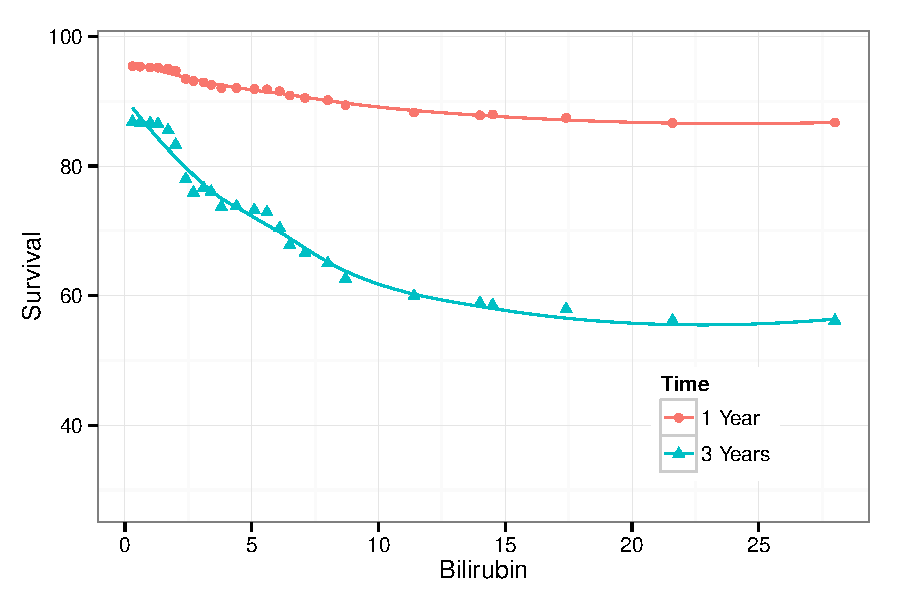
\includegraphics[width=.9\linewidth]{figures/pbc-partial-1} 

}



\end{knitrout}
\end{frame}
%==================================================================================
\begin{frame}
\frametitle{Partial Dependence}
\begin{knitrout}\footnotesize
\definecolor{shadecolor}{rgb}{0.969, 0.969, 0.969}\color{fgcolor}

{\centering 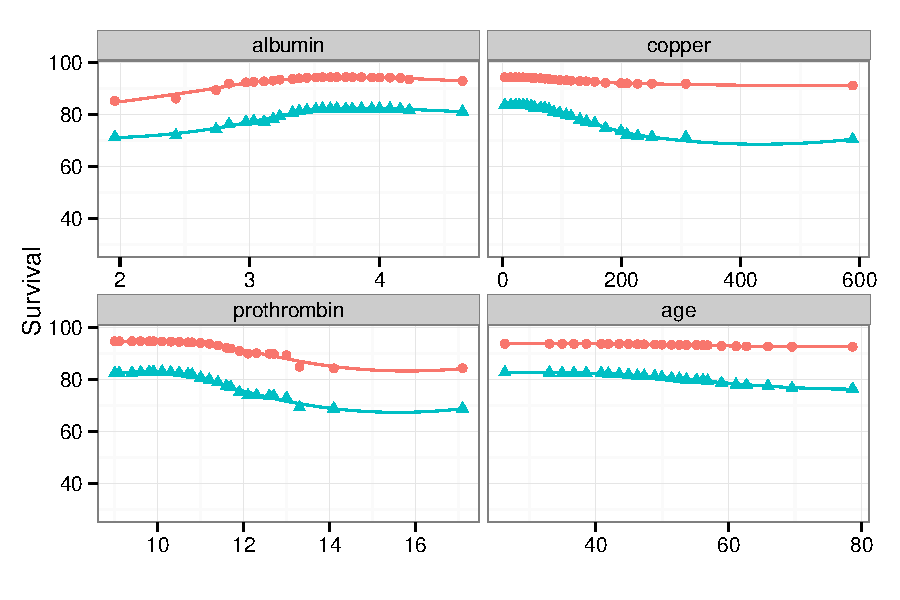
\includegraphics[width=.9\linewidth]{figures/partialpanel-1} 

}



\end{knitrout}
\end{frame}
%==================================================================================
\begin{frame}
\frametitle{Partial Dependence}

\begin{knitrout}\footnotesize
\definecolor{shadecolor}{rgb}{0.969, 0.969, 0.969}\color{fgcolor}

{\centering 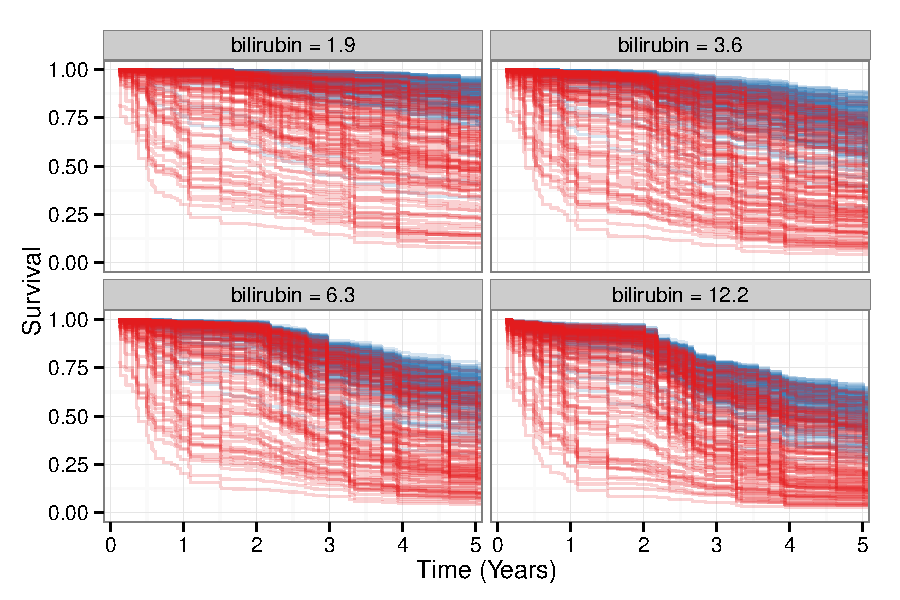
\includegraphics[width=.9\linewidth]{figures/rfs-nomo2-1} 

}



\end{knitrout}
\end{frame}

%==================================================================================
\begin{frame}
\frametitle{Partial Dependence}

\begin{knitrout}\footnotesize
\definecolor{shadecolor}{rgb}{0.969, 0.969, 0.969}\color{fgcolor}

{\centering 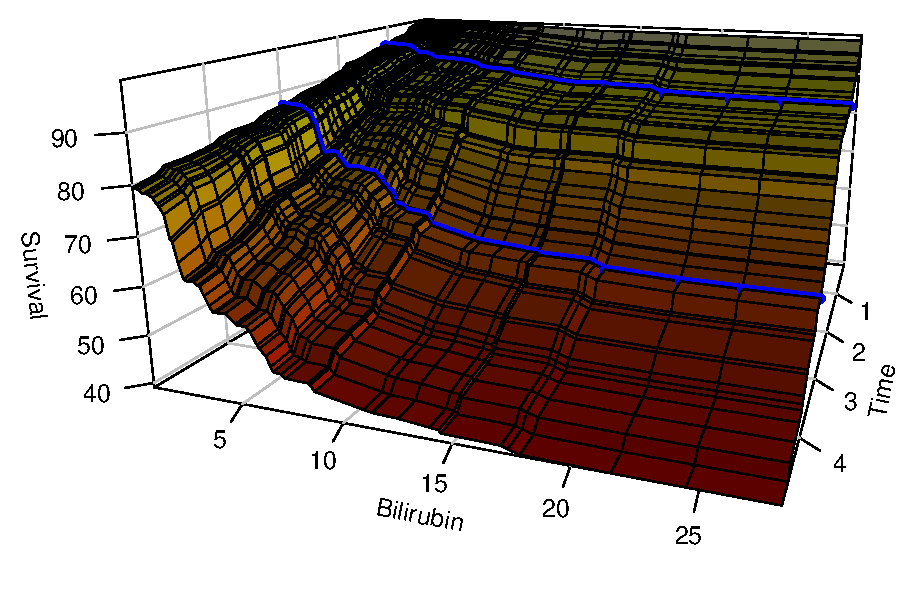
\includegraphics[width=.9\linewidth]{figures/pbc-timeSurface-1} 

}



\end{knitrout}
\end{frame}

\end{document}
